\documentclass[12pt,a4paper]{article}
\usepackage[utf8]{inputenc}
\usepackage[russian]{babel}
\usepackage[OT1]{fontenc}
\usepackage{amsmath}
\usepackage{amsfonts}
\usepackage{amssymb}
\usepackage{graphicx}
\usepackage{wrapfig}
\usepackage[left=2cm,right=2cm,top=2cm,bottom=2cm]{geometry}
\author{Николай Козырский}
\title{Лабораторная работа №6.1. Эффект Мессбауэра.}
\begin{document}
\maketitle
\section{Теория}
Зависимость интенсивности излучения атома от частоты описывается выражением:
\begin{equation}
I_\omega = I_0 \frac{\left( \Gamma /2 \right)^2}{\left( \Gamma /2 \right)^2 + (\omega - \omega_0)^2},
\end{equation}
иначе говоря, имеет Лоренцовскую зависимость с центром в $\omega_0$ и шириной на половине высоты, равной $\Gamma$.

Процесс, обратный испусканию, -- резонансное поглощение -- описывается той же зависимостью. Это значит, что эффективное сечение резонансного поглощения $\sigma(\omega)$ имеет вид
\begin{equation} \label{breitt-wigner}
\sigma(\omega) = \sigma_0 \frac{\left( \Gamma /2 \right)^2}{\left( \Gamma /2 \right)^2 + (\omega - \omega_0)^2},
\end{equation}
где $\sigma_0$ -- максимальное эффективное сечение поглощения, определяемое физикой процесса. Выражение  (\ref{breitt-wigner}) называется в ядерной физике формулой Брейта-Вигнера, и для бесспиновых частиц, вступающих в реакцию из s-состояния относительного движения, имеет вид
\begin{equation}
\sigma_{ab} = \pi \lambda_a^2 \frac{\Gamma_a \Gamma_b}{(E-E_0)^2 + (\Gamma / 2)^2},
\end{equation}
где $\Gamma_a$ -- ширина распада составного (возбужденного) ядра с испусканием налетающей частицы $a$ (упругое рассеяние), $\Gamma_b$ -- с испусканием другой частицы (неупругое рассеяние), $\Gamma = \Gamma_a + \Gamma_b$ полная ширина уровня, $\lambda_a$ -- длина волны бомбардирующей частицы. 

В случае резонанся сечение упругого рассеяния $\sigma_{aa}$ принимает вид:
\begin{equation}
\sigma_{aa} = 4 \pi \lambda_a^2 (\Gamma_a / \Gamma)^2.
\end{equation}
Это означает, что если энергетически возможно лишь упругое рассеяние, то максимальное сечение в резонансе равно 
\begin{equation}
\sigma_{aa} = \sigma_{aa,max} = 4 \pi \lambda_a^2.
\end{equation}
Сечение неупругого рассеяния максимально при $\Gamma_a = \Gamma_b = \Gamma /2$  и равно 
\begin{equation}
\sigma_{ab} = \sigma_{ab, max} = \pi \lambda_a^2
\end{equation}

В процессе испускания и поглощения $\gamma$-квантов излучающие и полгощающие свободные ядра элементов вследствие закона сохранения импульса приобретают часть энергии. Если энергия возбужденного уровня ядра $E_1^*$, энергия испускаемого $\gamma$-кванта $E_\gamma$, то 
\begin{equation}
E_\gamma = E_1^* - R,
\end{equation}
где $R$ -- кинетическая энергия отдачи.

При поглощении $\gamma$-кванта, имеющего энергию $E_\gamma$, таким же ядром оно также получает кинетическую энергию отдачи $R$, так что на возбуждение ядра будет затрачена энергия 
\begin{equation}
E_2^* = E_\gamma - R = E_1^* - 2R.
\end{equation}
Эффект Мессбауэра состоит в том, что если излучающее ядро не свободно, а находится в кристаллической решетке, то при определенных условиях поглощение и испускание $\gamma$-излучения с большой вероятностью происходят без потерь на отдачу, т.е. в спектре испускания (или поглощения) появляется несмещенная линия 
\begin{equation}
E_\gamma = E_1^* = E_2^*.
\end{equation}
Такое явление называется ядерной резонансной флуоресценцией или ядерным резонансным рассеянием (поглощением) или просто эффектом Мессбауэра. 
\section{Установка}
Блок схема экспериментальной установки приведена на рис. \ref{scheme}.

\begin{figure}[ht] \label{scheme} 
%\vspace{-5ex}  
 \center{\includegraphics[width=.7\linewidth]{scheme.png}}
\caption{Схема установки: Э -- эксцентрик, С -- сцинтилляционный кристалл, У -- усилитель, АА -- одноканальный амплитудный анализатор, ЭВМ -- персональный компьютер, ЗГ -- звуковой генератор, РД-09 -- двигатель с редуктором, ВСВ -- высоковольтный стабилизированный выпрямитель}
\end{figure}

Поглотителем служит оловянная фольга. Поглотитель укреплен в рамке, приводимой в движение кулачковым механизмом. Форма эксцентрика выбрана так, чтобы движение поглотителя происходило с постоянной скоростью.

\section{Ход работы} 

\begin{enumerate}

\item Снять распределение числа испускаемых гамма-квантов по их энергиям. По полученному распределению подобрать настройки анализатора импульсов так, чтобы детектировались только гамма-кванты с энергией 23.8 кЭв.

\item Получить зависимость поглощения от относительной скорости поглотителя. В работе исследуются 4 образца: 3 образца олова различной толщины, и один образец оксида олова $SnO_2$.

\end{enumerate}

\section{Обработка результатов}

\begin{enumerate}

\item Калибровка:
\begin{figure}[ht!]
 \center{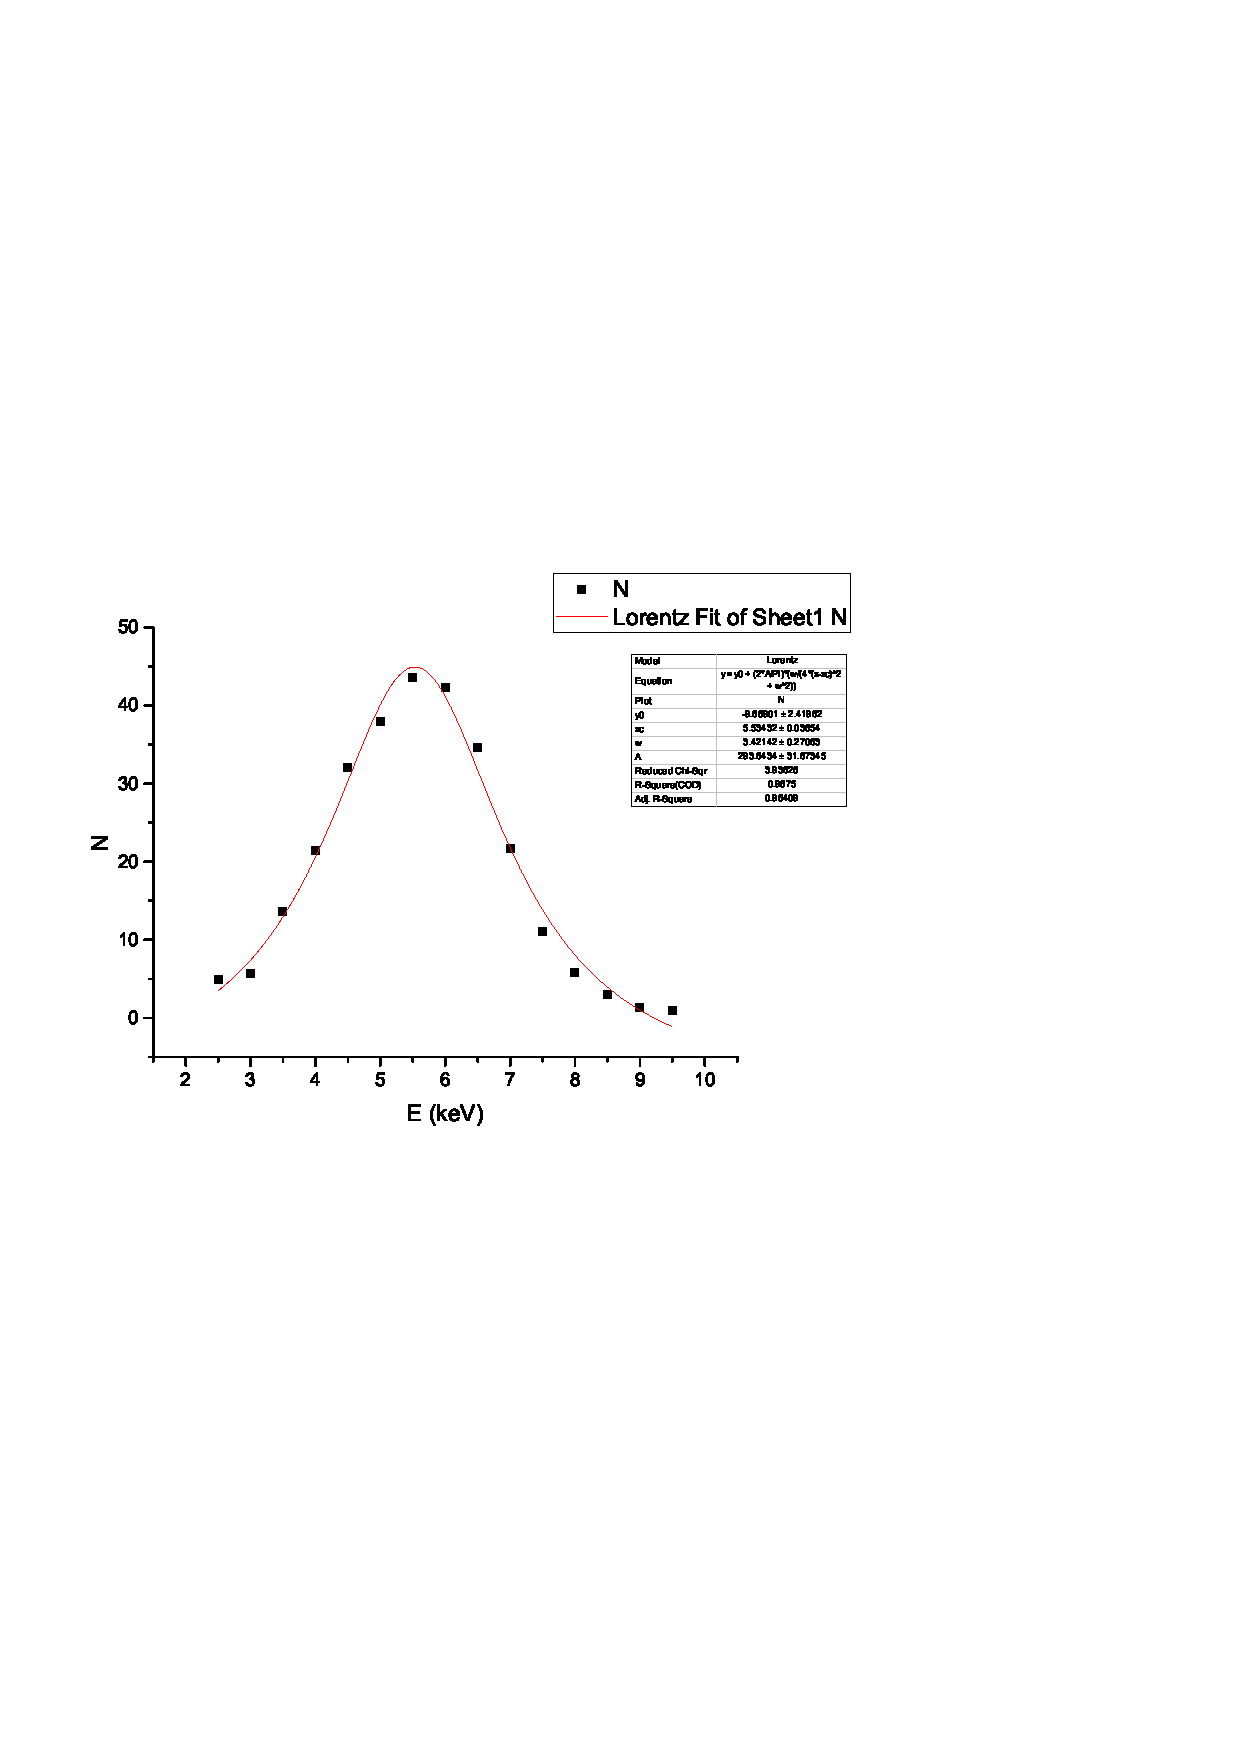
\includegraphics[width=\linewidth]{graph.pdf}}
\caption{Калибровочный график}
\end{figure}

По результатам калибровки на анализаторе сигналов выбраны рабочие пределы от 2В до 10В.

\newpage

\item Образец олова толщиной 100мкм (образец 1):

\begin{figure}[ht!]
 \center{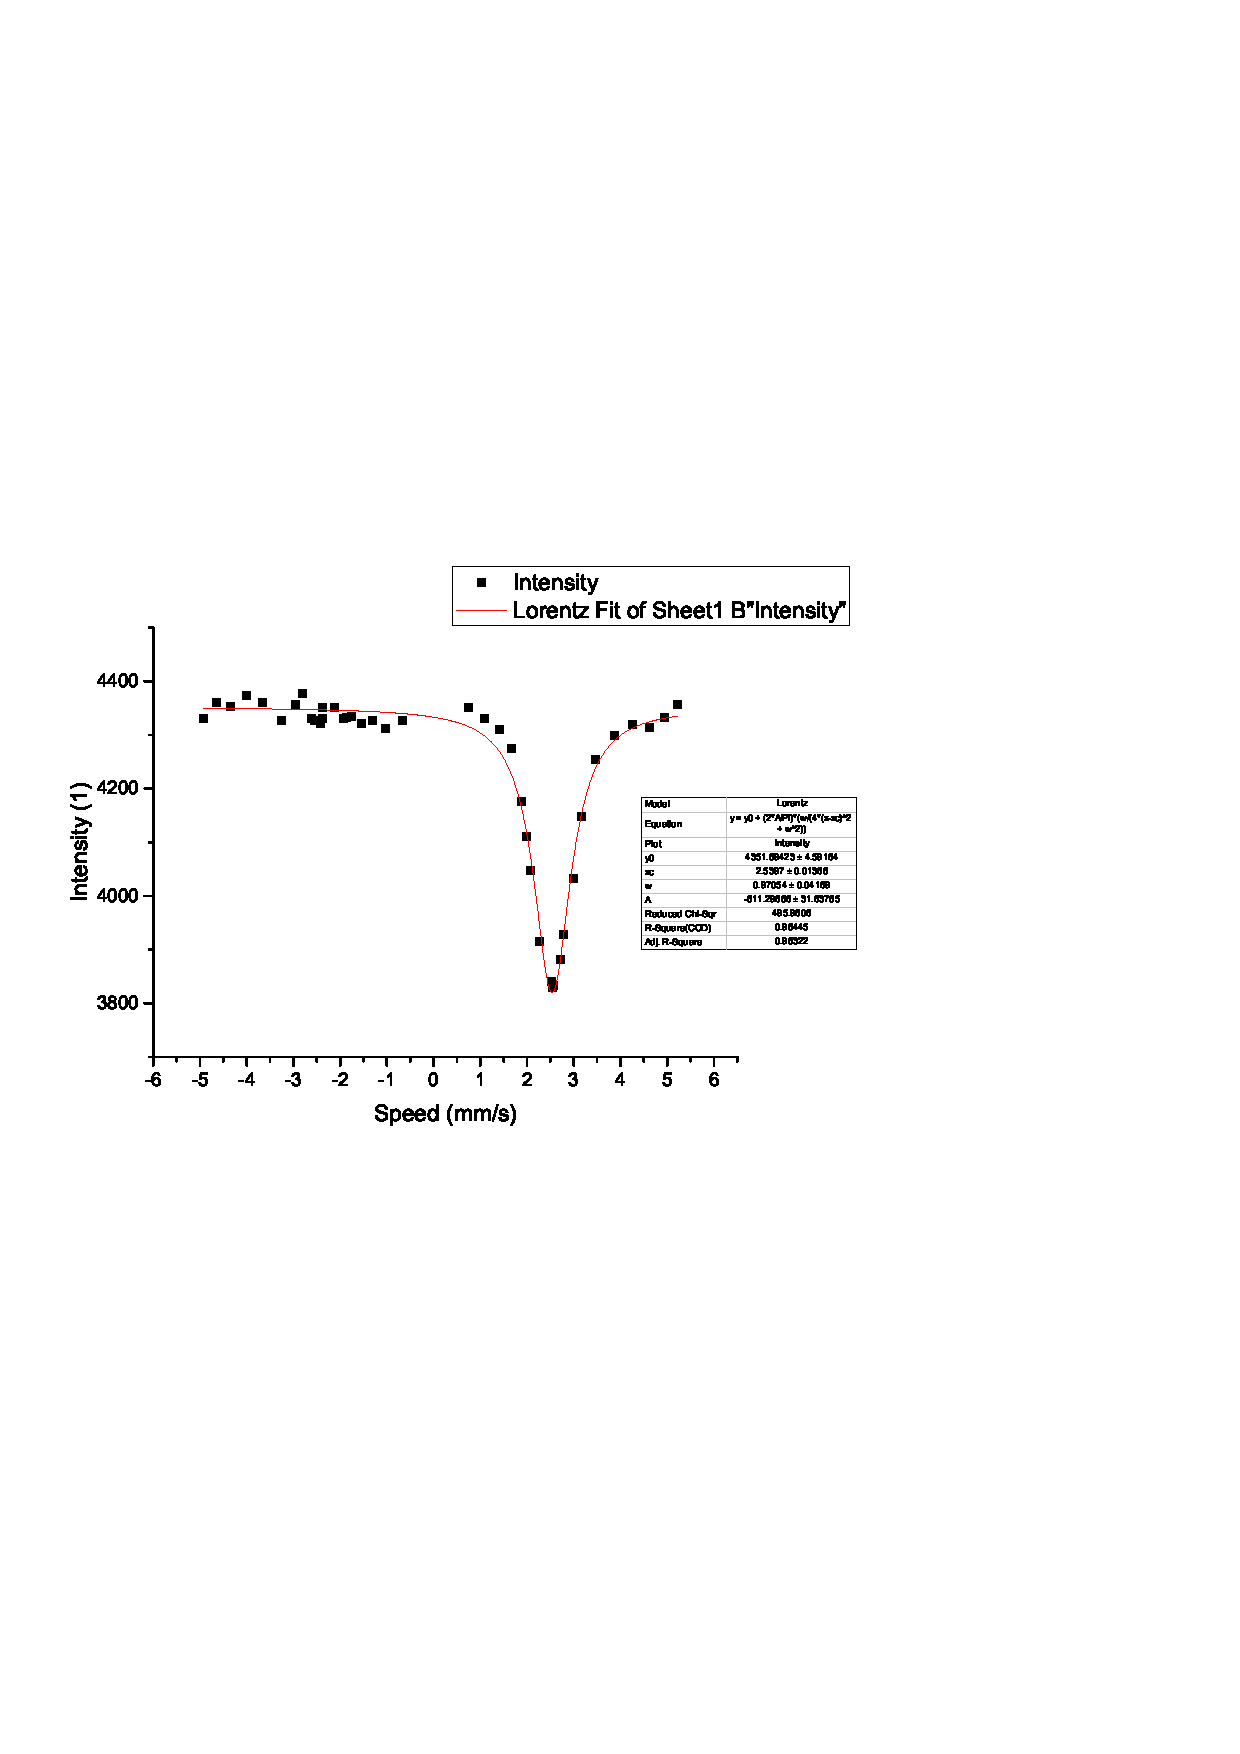
\includegraphics[width=.65\linewidth]{graph1.pdf}}
\caption{Олово 100мкм}
\end{figure}

Амплитуда: 
\begin{equation*}
\epsilon = \frac{4350 - 3850}{4350} \cdot 100\% = 11.5 \%
\end{equation*}
Хим. сдвиг: $2.54 \pm 0.01 mm/s = 15.88 \pm 0.06 \cdot 10^{-8} eV$ \\
$\Gamma_{exp} = 1.94 \pm 0.08 mm/s = 12.1 \pm 0.5 \cdot 10^{-8} eV$ \\


\item Образец олова толщиной 200мкм (образец 2):

\begin{figure}[ht!]
 \center{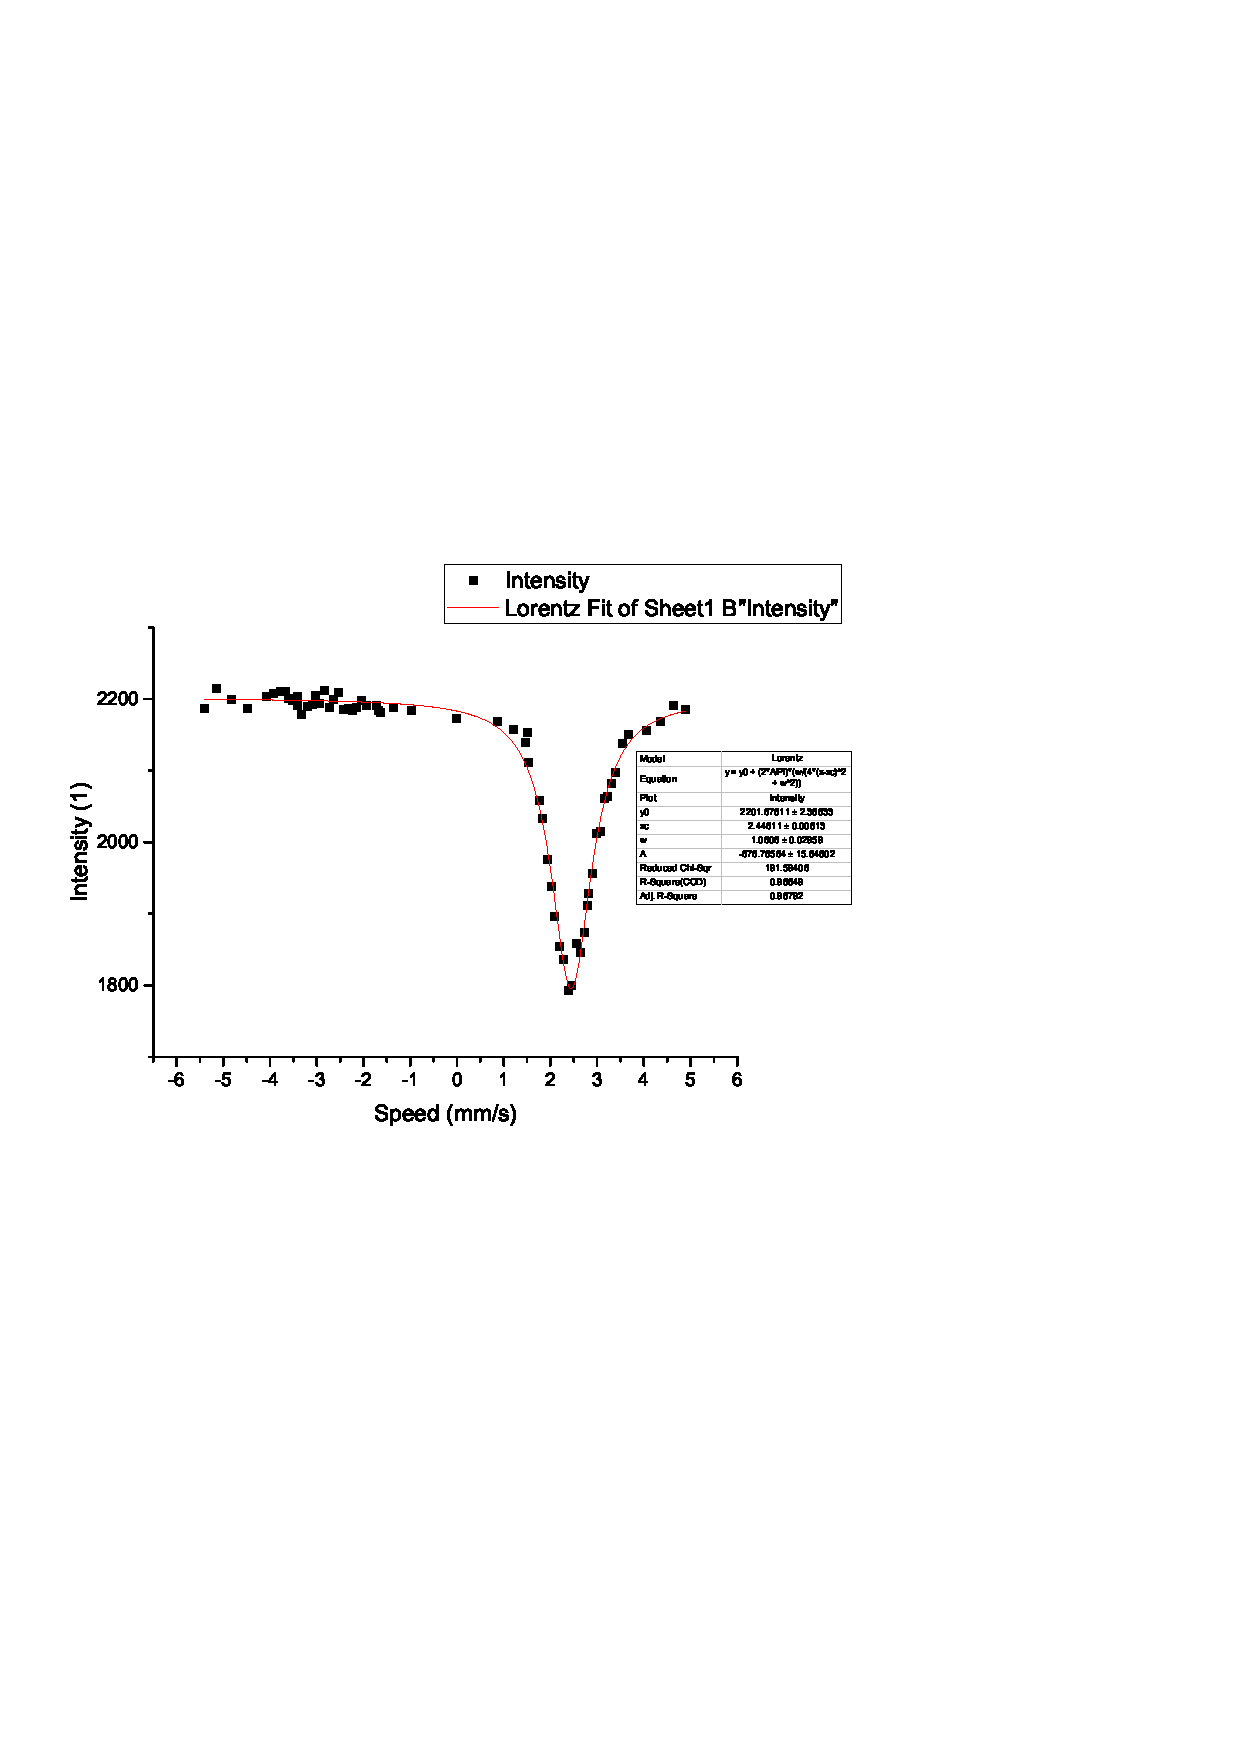
\includegraphics[width=.65\linewidth]{graph2.pdf}}
\caption{Олово 200мкм}
\end{figure}


Амплитуда: 
\begin{equation*}
\epsilon = \frac{2200 - 1800}{2200} \cdot 100\% = 18.2 \%
\end{equation*}
Хим. сдвиг: $2.45 \pm 0.01 mm/s = 15.32 \pm 0.06 \cdot 10^{-8} eV$ \\
$\Gamma_{exp} = 2.12 \pm 0.06 mm/s = 12.3 \pm 0.4 \cdot 10^{-8} eV$ \\

\newpage

\item Образец $SnO_2$ (образец 4):

\begin{figure}[ht]
 \center{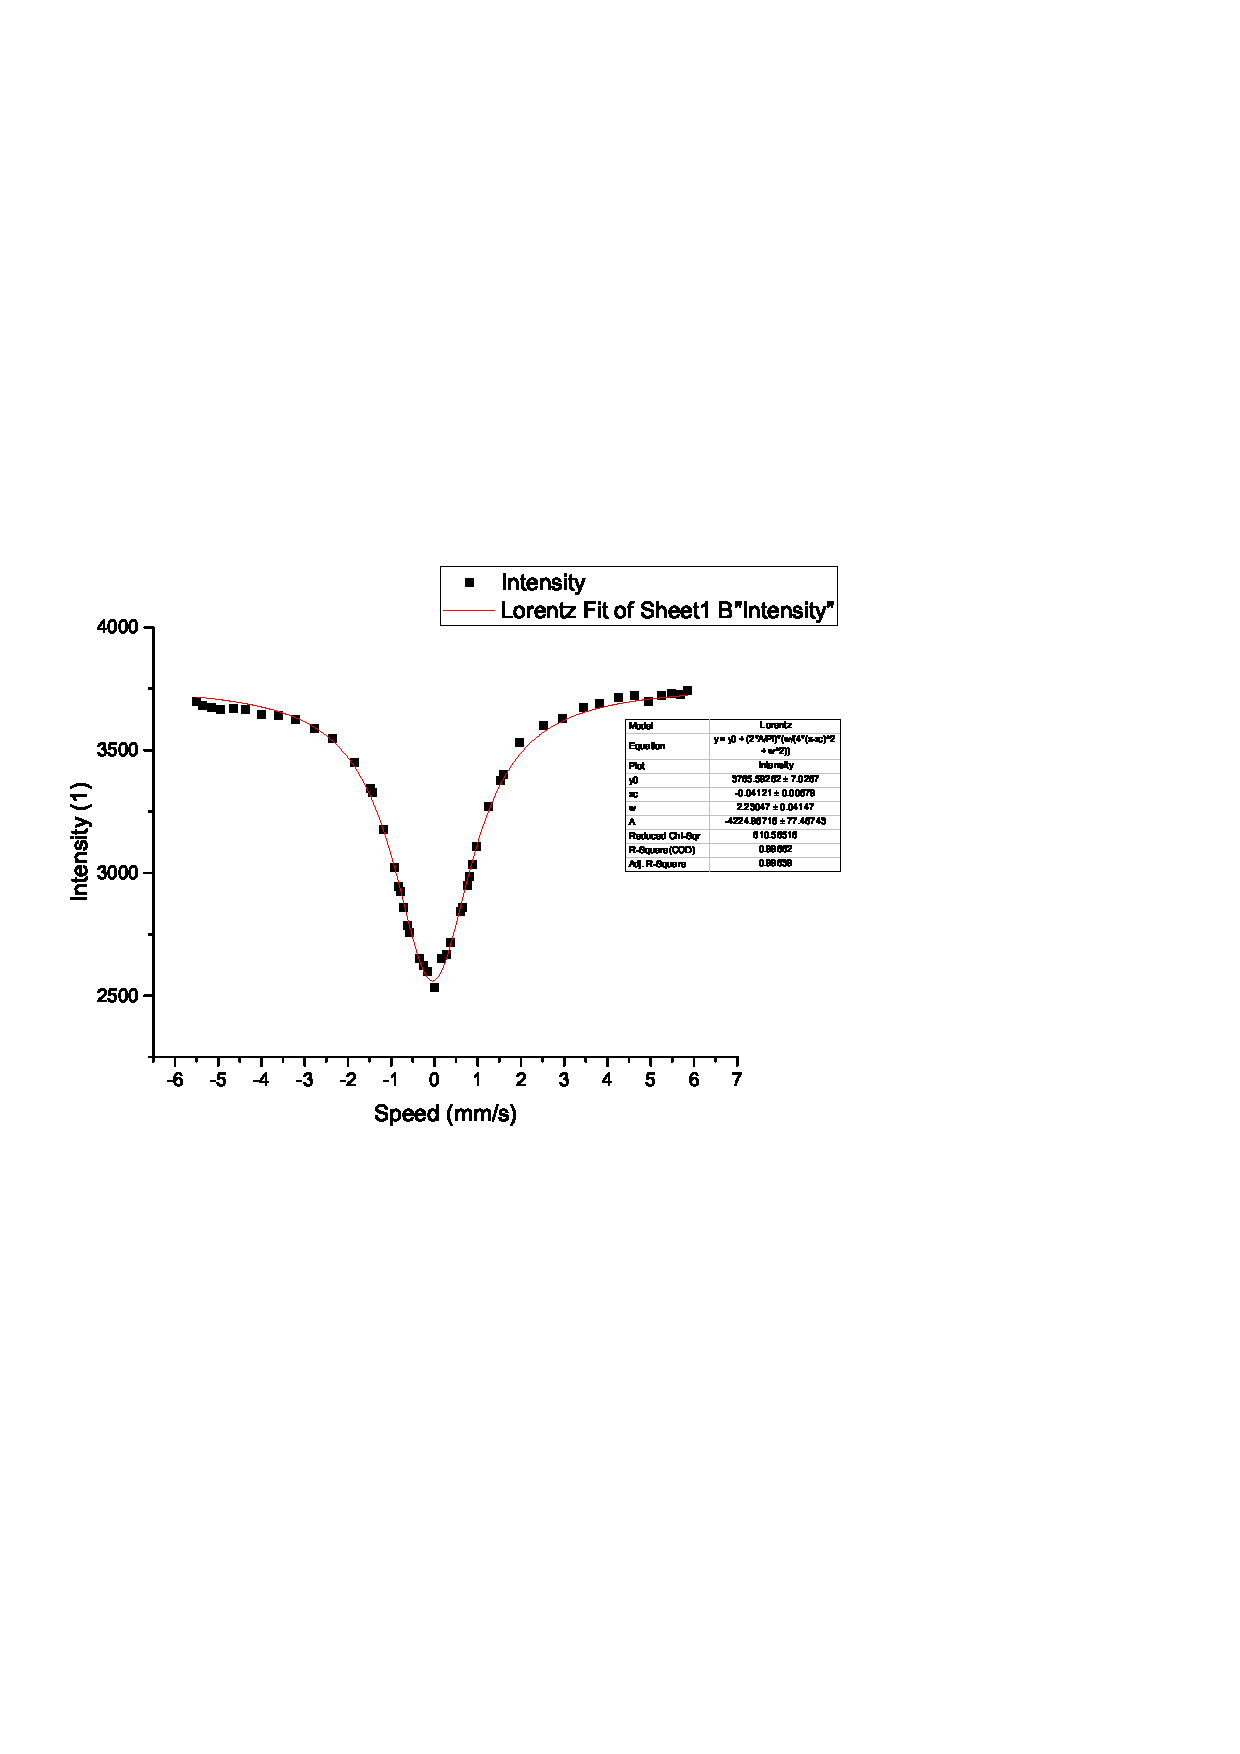
\includegraphics[width=.7\linewidth]{graph4.pdf}}
\caption{$SnO_2$}
\end{figure}
Амплитуда: 
\begin{equation*}
\epsilon = \frac{3750 - 2500}{3750} \cdot 100\% = 33.3 \%
\end{equation*}
Хим. сдвиг: $-0.04 \pm 0.01 mm/s = 0.25 \pm 0.06 \cdot 10^{-8} eV$ \\
$\Gamma_{exp} = 1.94 \pm 0.08 mm/s = 27.9 \pm 0.3 \cdot 10^{-8} eV$ \\

\end{enumerate}

\section{Обсуждение результатов}
Полученные величины $\Gamma_{exp}$ по порядку величины совпадают со значениями, приведенными в учебнике. Полученные экспериментальные данные с большой степенью точности ($R^2 \equiv 0.99$) описываются кривой Лоренца. Погрешности полученных значений $\Gamma_{exp}, \epsilon$ и хим.сдвига лежат в пределах 5 \%.

\section{Вывод}
С помощью метода доплеровского сдвига мессбауэрских линий испускания и поглощения были исследованы резонансное поглощение гамма-квантов испускаемыми ядрами олова в соединении $BaSnO_3$ при комнатной температуре. Был определен максимум резонансного поглощения, его величина, а также экспериментальная ширина линии $\Gamma_{exp}$.
Результаты измерений приведены в таблице ниже:
\begin{center}
\begin{tabular}{cccc}
Образец & Амплитуда(\%) & Хим.сдвиг(эВ $\cdot 10^{-8}$) & $\Gamma$(эВ $\cdot 10^{-8}$) \\
1 & $11.5$ & $ 15.88 $ & $ 12.1 $  \\
2 & $18.2$ & $ 15.32 $ & $ 12.3$ \\
4 & $33.3$ & $ 0.25 $   & $ 27.9 $ \\
\end{tabular}
\end{center}

%\end{enumerate}

\end{document}